\subsection{service}
\label{subsec:service}

\begin{figure}[H]
  \centering
  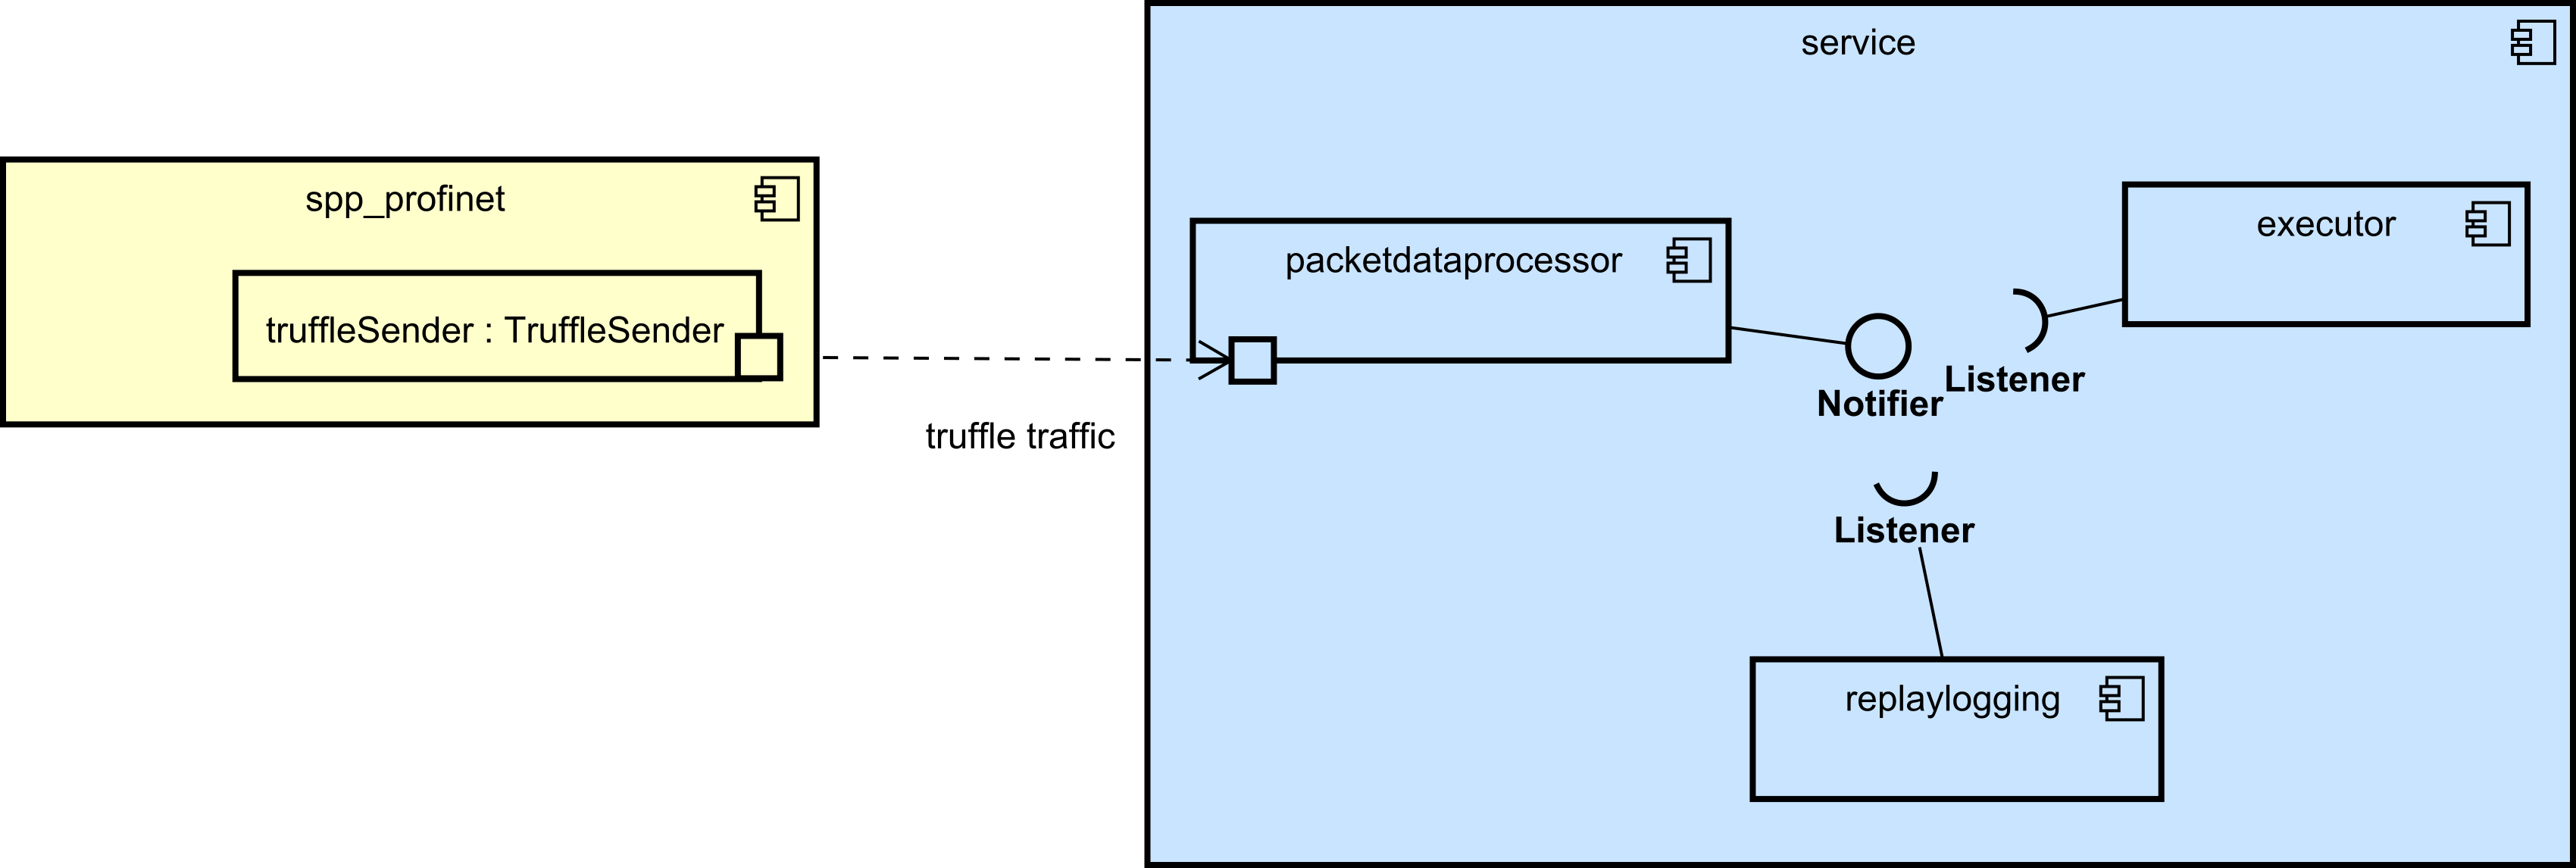
\includegraphics[width=\textwidth]{../diagramimages/service.png}
  \caption{service-Package}
\end{figure}

\medskip
Im service-Package befinden sich alle kontinuierlich laufenden Threads von \gls{programname},
mit Ausnahme von \hyperref[subsec:view]{view}, das in einem eigenen Thread zur verzögerungsfreien Darstellung läuft, und dem
main-Thread. Jedes Unterpackage kapselt dabei genau eine selbständig laufende Funktionalität. In den folgenden Abschnitten ist erklärt, was genau die Unterpackages packetdataprocessor, replaylogging und executor machen.

    \subsubsection{packetdataprocessor}
    \label{subsubsec:truffleprocessor}

    Der packetdataprocessor-Service läuft konstant im Hintergrund, in einem eigenen Thread,
    und empfängt die im \gls{sppname} erstellten Truffles.
    Diese werden in ein Java-Truffle-Objekt gepackt, welches dann wiederum von dem
    \textit{TruffleReceiver} in ein Command gesteckt wird. Da der \textit{TruffleReceiver}
    ein \gls{notifier} ist, verschickt er den Command an
    alle registrierten \gls{listener}, sodass der CommandExecutor die Commands bekommt. Dort werden sie
    dann ausgeführt.

    \clearpage
    \begin{sidewaysfigure}
      \centering
      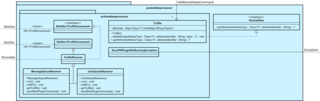
\includegraphics[width=\textwidth]{../diagramimages/packetdataprocessor.png}
      \caption{packetdataprocessor-Package}
    \end{sidewaysfigure}
    \clearpage

    \subsubsection{replaylogging}
    \label{subsubsec:replaylogging}

    Der replaylogging-Service besteht aus zwei Hauptaufgaben, die jeweils in ihrem eigenen Thread laufen.
    Die erste ist der \textit{ReplayLogSaveService} und kümmert sich um das Speichern des aktuellen
    Graphen. Die zweite ist der \textit{ReplayLogLoadService} und kümmert sich um das
    Wiederherstellen eines gespeicherten Graphen.
    \newline
    \newline
    Der \textit{ReplayLogSaveService} läuft konstant im Hintergrund und empfängt alle
    vom \textit{TruffleReceiver} verschickten Commands. Diese werden alle X
    Sekunden (vom Benutzer festlegbar) komprimiert und in eine Liste gepackt.
    Komprimiert heißt, dass viele Commands, die dasselbe tun, in einen einzelnen Command
    gepackt werden. Zusätzlich zu den Commands wird auch noch ein Snapshot
    von dem aktuellen Graphen angefertigt, der dann zusammen mit der erstellten
    Command-Liste in ein ReplayLog-Objekt gepackt wird. Dieses
    ReplayLog-Objekt wird dann serialisiert und gespeichert.
    \newline
    \newline
    Diese Logs können zu einem späteren Zeitpunkt wieder geladen werden, um den
    Graphen wiederherzustellen. Dazu ist der \textit{ReplayLogLoadService} da. Wenn
    der Nutzer die Replayfunktion aktiviert, fängt der ReplayLogLoadService an, die
    ReplayLogs zu laden. Dann wird in der View der Snapshotgraph angezeigt
    und die gespeicherten Commands aus dem ReplayLog werden auf
    diesem Snapshot ausgeführt. Der ReplayLogLoadService kontrolliert somit die
    Wiedergabe des alten Graphen und kann sogar zwischen Snapshots hin und her
    springen (momentan nicht zwischen einzelnen Commands, da diese keine undo-
    und redo-Funktion besitzten).
    \newline
    \newline
    Der ReplayLogLoadService läuft in seinem eigenen Thread, weil er sich darum
    kümmert, dass immer genügend Daten im Speicher liegen. In anderen Worten, er
    buffert die ReplayLogs vor, damit der Graph bei dem Benutzer flüssig
    abgespielt wird.

    \clearpage
    \begin{sidewaysfigure}
      \centering
      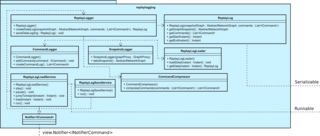
\includegraphics[width=\textwidth]{../diagramimages/replaylogging.png}
      \caption{replaylogging-Package}
    \end{sidewaysfigure}
    \clearpage

    \subsubsection{executor}
    \label{subsubsec:executor}

    \begin{figure}[H]
      \centering
      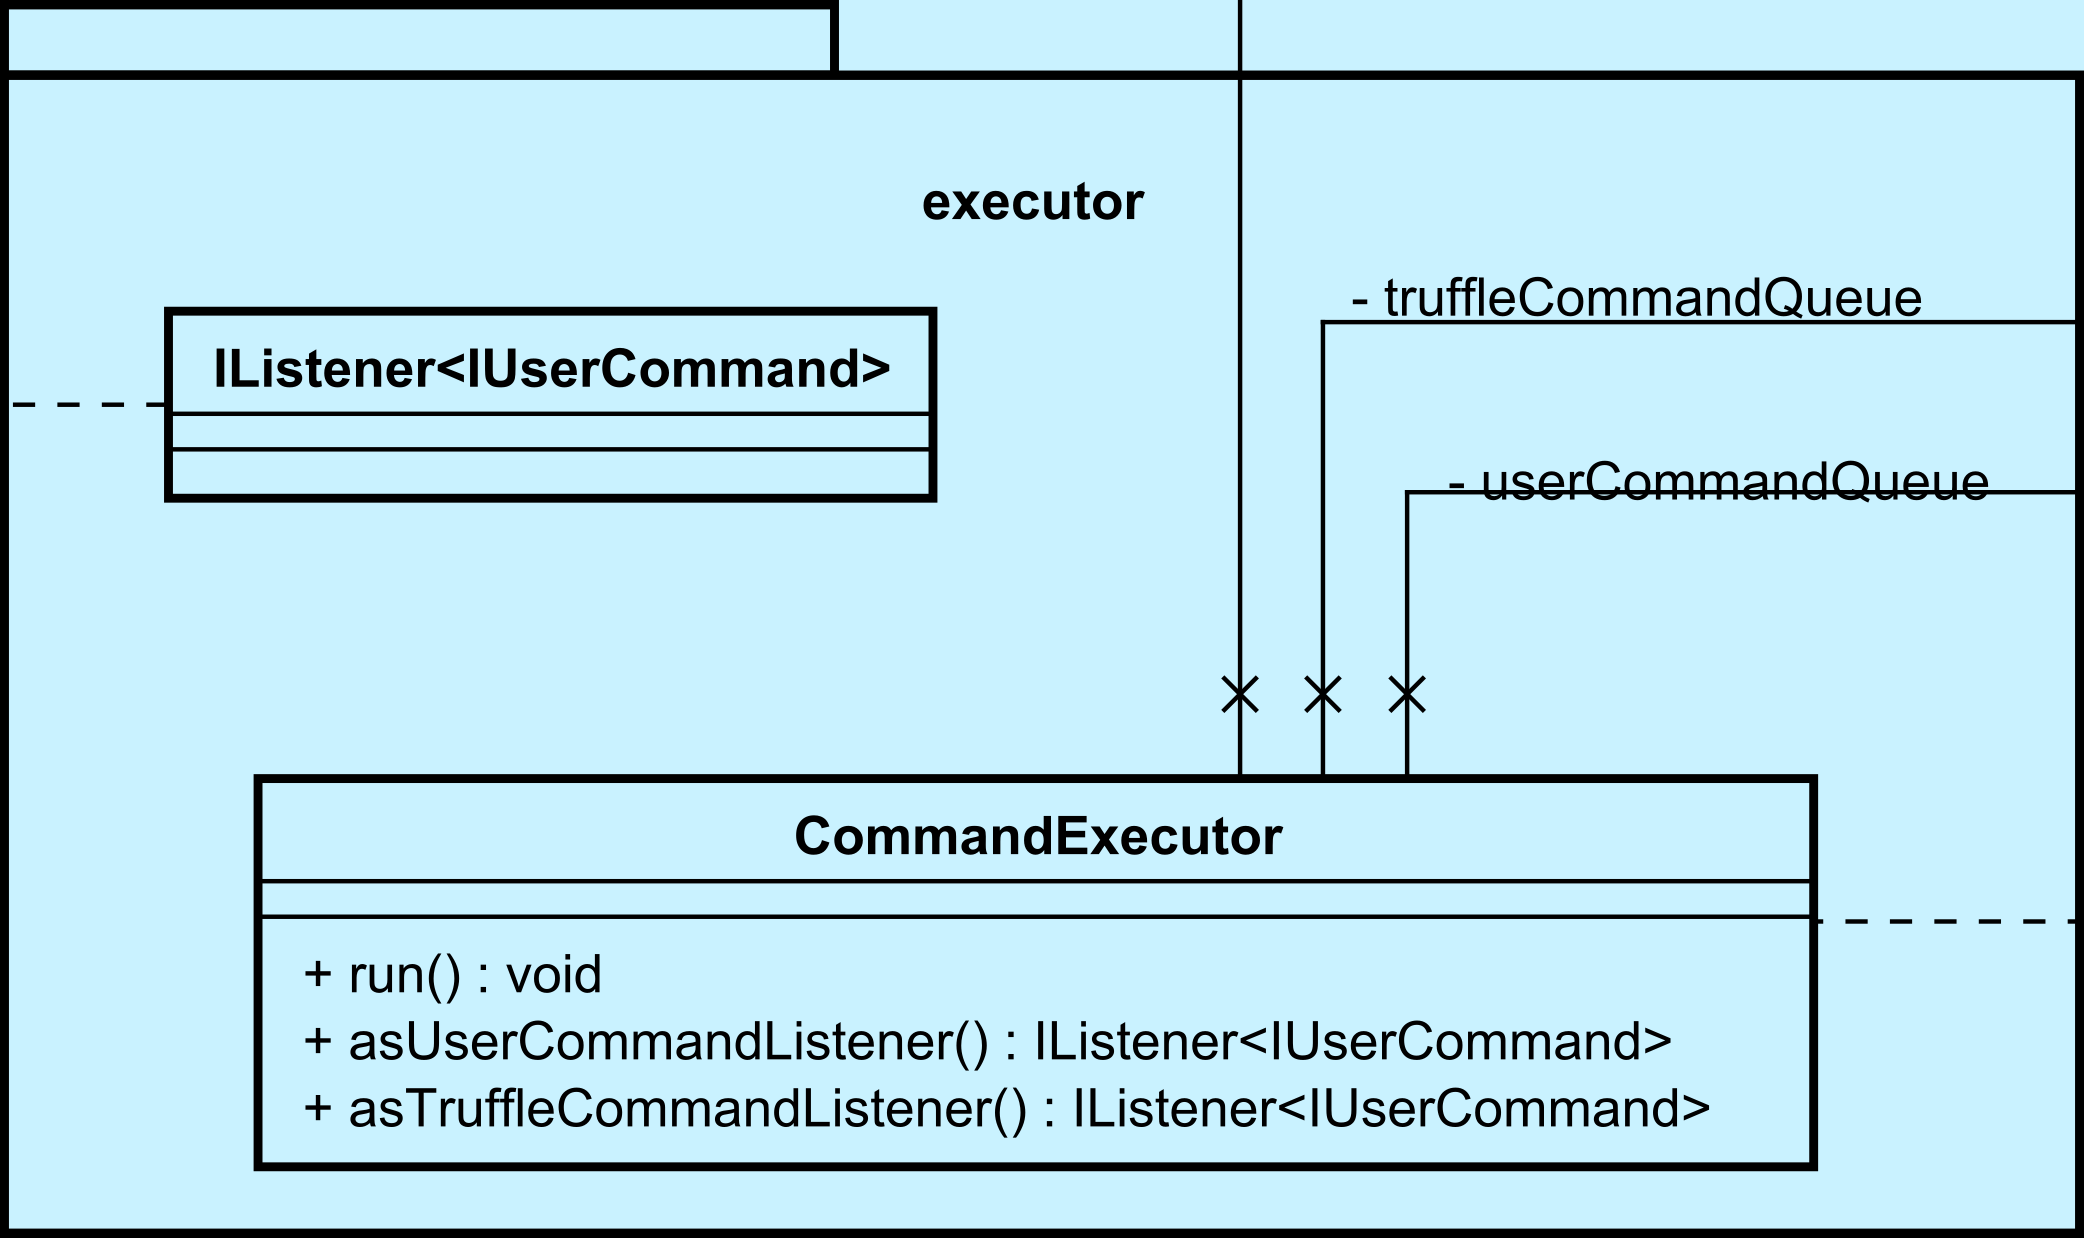
\includegraphics[width=\textwidth]{../diagramimages/executor.png}
      \caption{executor-Package}
    \end{figure}

    \medskip
    Der executor-Service läuft ebenfalls konstant im Hintegrund in seinem
    eigenen Thread. Er ist ein \gls{listener}, der sowohl bei dem TruffleReceiver aus dem
    \hyperref[subsubsec:packetdataprocessor]{packetdataprocessor}-Package als
    auch bei den view-Controllern aus dem \hyperref[subsec:view]{view}-Package
    registriert ist. D.h., er bekommt, wie das \hyperref[subsubsec:replaylogging]{replaylogging},
    alle \hyperref[subsubsec:trufflecommand]{TruffleCommands} und führt diese
    dann auf dem aktuellen Model aus.
    \newline
    \newline
    In \gls{programname} gibt es zwei Instanzen vom Executor. Die erste bearbeitet
    den aktuellen Graphen und die zweite bearbeitet die Snapshot-Instanz, falls
    eine existiert. So kann der aktuelle Graph auf dem neuesten Stand bleiben, während
    der Benutzer gleichzeitig einen alten Graphen aus
    ReplayLogs rekonstruiert anschaut.
